\documentclass[landscape,twocolumn,a4]{article}
\usepackage[utf8]{inputenc}
\usepackage[usenames,dvipsnames,svgnames,table]{xcolor}
\usepackage{graphicx}
\usepackage{float}

\title{Receita de Omelete}
\author{Rafael Lima}
\date{May 2014}

\definecolor{laranjEu}{rgb}{1.00,0.4980,0.000}

\pagestyle{empty}

\begin{document}

\begin{center}Receita De Omelete\end{center}

\begin{figure}[H]
\centering
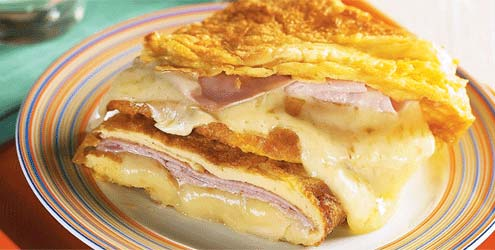
\includegraphics[width=8cm]{./img/receita-omelete-recheada}
\label{fig:my_label}
\end{figure}

\vspace{1cm}

\begin{table}[H]
\centering
\begin{tabular}{lc}
Dificuldade & Fácil\\
Rendimento & 4 porções\\
Tempo de Preparo & 30min\\
Calorias & 204 por porção\\
\end{tabular}
\end{table}

\newpage

\begin{center}
\color{laranjEu}
\rule{3cm}{1mm}\hspace{5mm}{
INGREDIENTES
}\hspace{5mm}\rule{3cm}{1mm}
\end{center}

Omelete:
\begin{table}[H]
\centering
\begin{tabular}{lc}
\hline
 4 Ovos Grandes & \parbox[c]{2cm}{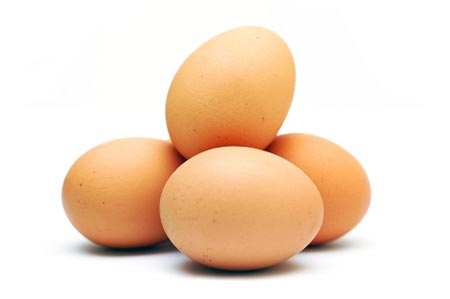
\includegraphics[width=2cm]{img/ovos.jpg}}\\
 Sal a gosto & \parbox[c]{2cm}{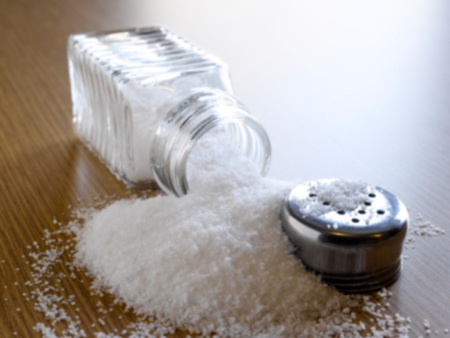
\includegraphics[width=2cm]{img/sal.jpg}}\\
 $\frac{1}{4}$ xícara de chá de Creme de Leite & \parbox[c]{2cm}{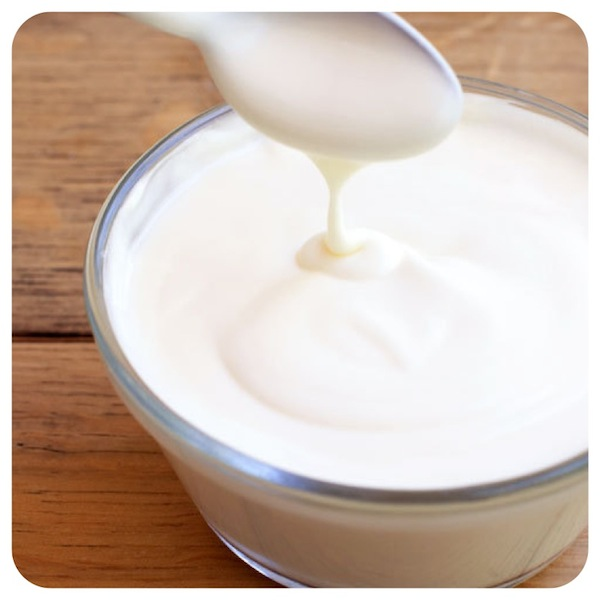
\includegraphics[height=2cm]{img/cremeLeite.jpg}}\\
 7 fatias de Queijo & \parbox[c]{2cm}{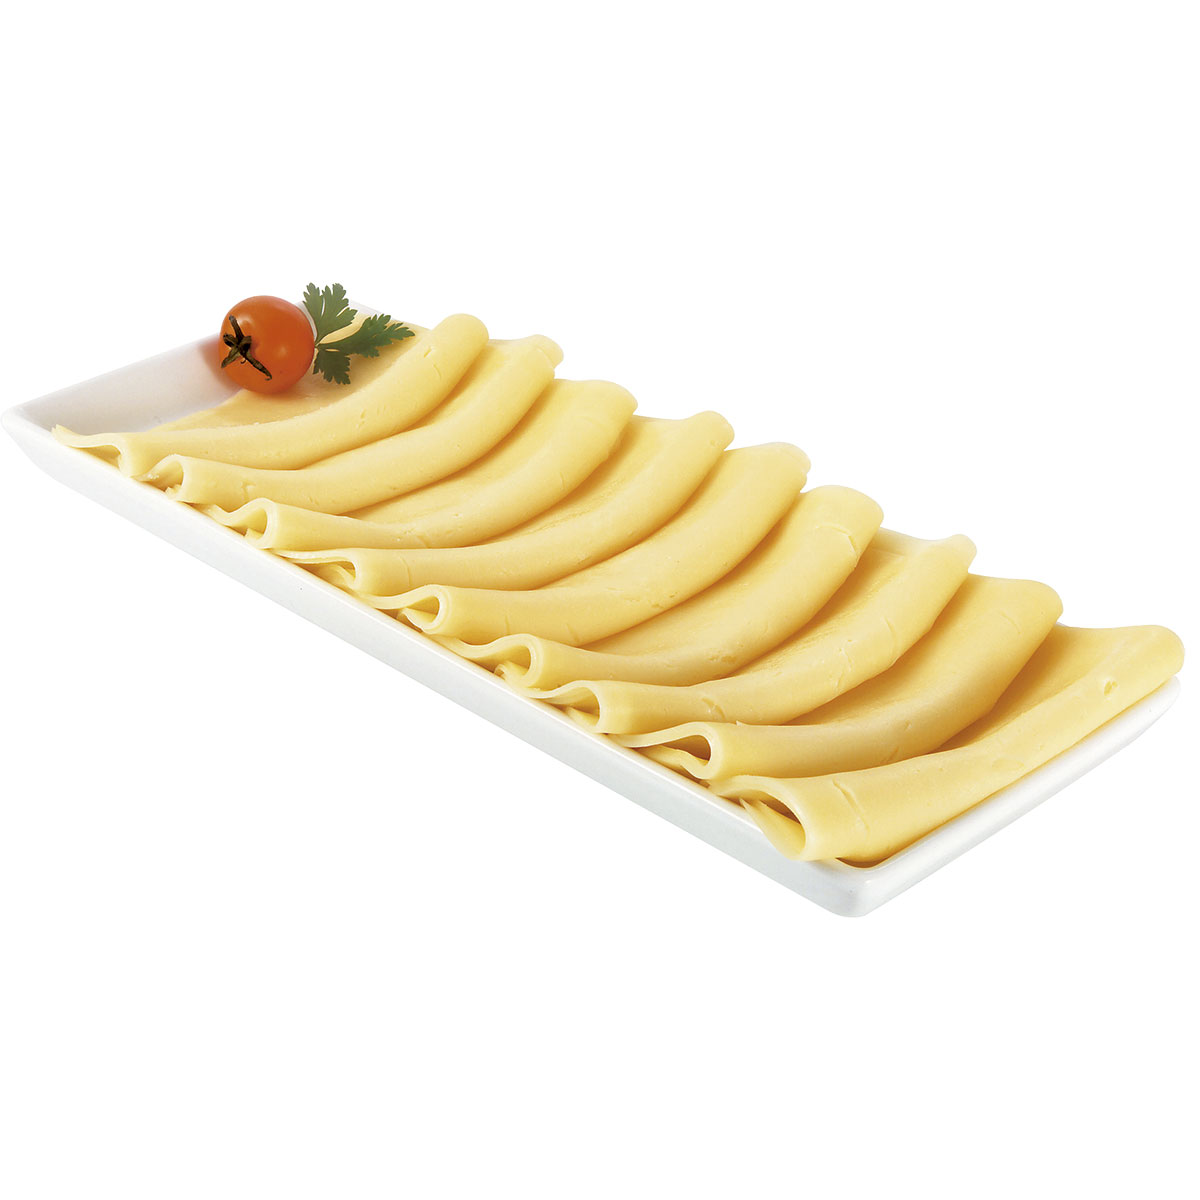
\includegraphics[width=2cm]{img/mussarela.jpg}}\\
 4 fatias de Presunto & \parbox[c]{2cm}{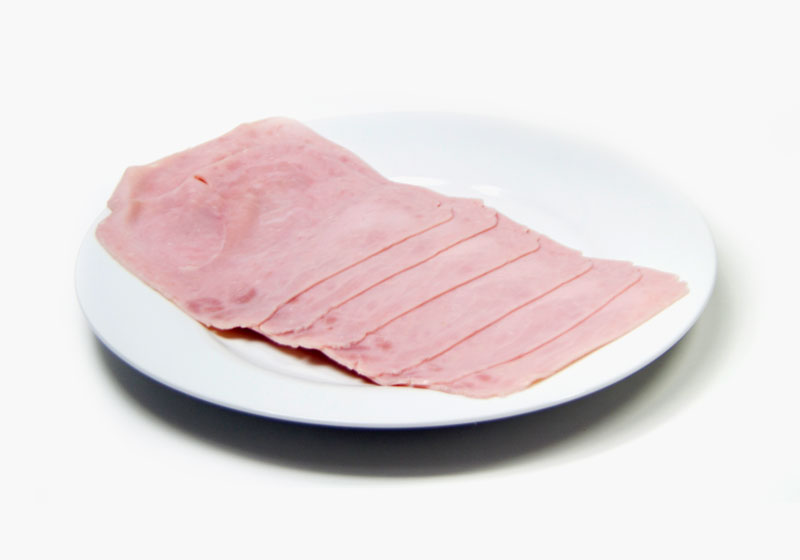
\includegraphics[width=2cm]{img/presunto.jpg}}\\
 \hline
\end{tabular}
\end{table}

\newpage
Para untar:
\begin{table}[H]
\centering
\begin{tabular}{lc}
\hline
 1 colher de chá de Óleo & \parbox[c]{2.1cm}{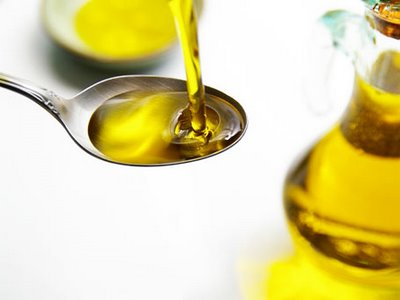
\includegraphics[width=2cm]{img/oleo.jpg}}\\
 1 xícara de chá de Água & \parbox[c]{2.1cm}{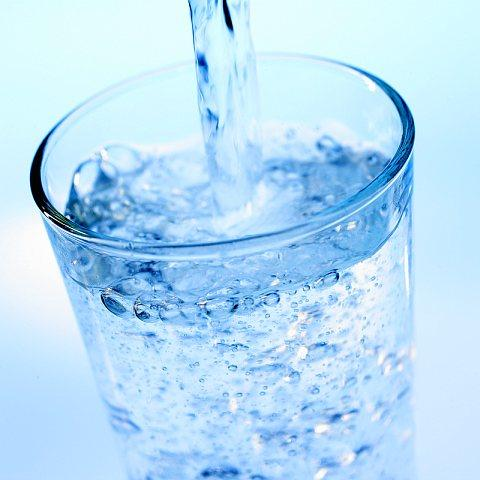
\includegraphics[width=2cm]{img/agua.jpg}}\\
 4 xícara de chá de Açucar & \parbox[c]{2.1cm}{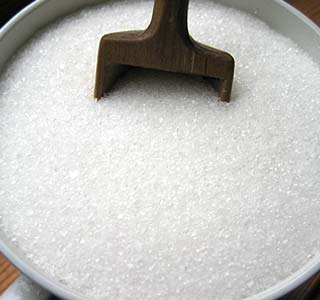
\includegraphics[width=2cm]{img/acucar.jpg}}\\
 2 xícara de chá de Coco Ralado & \parbox[c]{2.1cm}{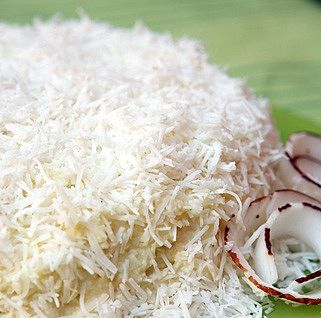
\includegraphics[width=2cm]{img/coco.jpg}}\\
 \hline
\end{tabular}
\end{table}

\newpage
\begin{center}
\color{laranjEu}
\rule{3cm}{1mm}\hspace{5mm}{
PROCEDIMENTOS
}\hspace{5mm}\rule{3cm}{1mm}
\end{center}

\begin{enumerate}
	\item Bata os ovos na batedeira com sal.
	\item Junte o creme de leite e continue batendo por mais dois minutos.
	\item Unte uma frigideira antiaderente com um pouco de óleo e aqueça bem.
	\item Ponha a mistura de ovos e incline um pouco a frigideira para espalhar por igual. \item Tampe e deixe cozinhar em fogo baixo por dois minutos.
	\item Vire a omelete, distribua as fatias de mussarela e presunto por cima.
	\item Dobre ao meio, tampe a frigideira e cozinhe até o queijo derreter. Sirva em seguida.
\end{enumerate}

\end{document}
